Prjón og hönnun var unnin í nánu samstarfi tölvunarfræðinema og fatahönnuðar og lagði mesta áherslu á hugmyndir útfærsla, möguleika í prjóni auk þess að leggja áherslu á framleiðslu á vélprjóni á \textit{Passap 6000}. Með  samstarfinu varð niðurstaðan áhugaverðari og náði betur til hönnuða en ella. 

\subsubsection{Hlutverk fatahönnuðar}
Hlutverk fatahönnuðsins var því að veita fagurfræðilega leiðsögn frá sjónarhorni hönnuða. Afurðin var jafnvægi milli skapandi hönnunar, hagnýtra takmarkana vélarinnar og þess sem hægt var að kóða á þessum skamma tíma. 

Þar sem möguleikar uppfærðrar prjónavélar voru óljósir við upphaf verkefnisins var erfitt að sjá fyrir lokaútkomu í hönnun. Því var hönnunarferlið sífellt á breytingu en lagði áherslu á möguleikana í stað þess að einblína á loka útkomu hönnunar. 

\subsubsection{Hönnunarhugsun}
Hönnuður styður sig við hugmyndir hönnunar hugsunar (e. \textit{Design Thinking}) sem gjarnan er kennd við hönnunardeild Stanford háskóla í Kaliforníu \cite{designthinking}.  Þau skilgreina 5 stig hönnunar:
\begin{enumerate}
    \item \textbf{Samkennd} (e. \textit{Empathize}): hvers vegna er hönnunin mikilvæg,
    \item \textbf{Þarfir} (e. \textit{Define}): þarfir afmarkaðar,
    \item \textbf{Hugmyndir} (e. \textit{Ideate}): ýmsar aðferðir skoðaðar,
    \item \textbf{Frumgerð} (e. \textit{Prototype}): hugmyndir afmarkaðar og að lokum
    \item \textbf{Prófun} (e. \textit{Test}) en þar eru hugmyndir kynntar til þess að fá viðbrögð frá ólíkum aðilum.
\end{enumerate}
Hönnuður náði  4 stigum hönnunar enn sem komið er en næsta og jafnframt afurð síðasta stigsins verður kynnt á Hönnunarmars.

\subsubsection{Prjón með mörgum litum}
Prufað var að prjóna með tveimur litum og kóðinn nýttur til þess að senda á prjónavélina texta eða mynstur í tveimur litum, sjá myndir \ref{fig:peacock}-\ref{fig:repeat} af fyrstu prufum sumarsins. Með uppfærslu var hægt að prjóna með þremur litum og að lokum fjórum. Útkomurnar urðu sífellt áhugaverðari og flóknari. 

Misvel gekk þó að prjóna og í byrjun áttum við erfitt með að prjóna með 4 litunum. Þá voru prjónaðar 8 umferðir á aftara borðinu fyrir hverja eina umferð á því fremra. Þetta olli miklum vandræðum en með breyttu prjóni, sem aðeins prjónar aðra hverja lykkju að aftan gekk betur að nota alla fjóra litina. Þá  voru prjónaðar 4 umferðir að aftan fyrir hverja eina að framan. 
\subsubsection{Áskoranir og betrumbætur í prjóni}
Stöðugt var verið að betrumbæta kóðana sem auðveldaði fyrir okkur prjónið. Margar prufurnar voru prjónaðir með handafli en þegar líða fór á sumarið tók mótorinn loksins við. Ýmis mannleg mistök áttu sér stað og gleymist reglulega að passa að setja strekkjarana aftur á þegar búið var að laga það sem laga þurfti. Þetta olli því að garnið komst illa á nálarnar sem verður til þess að sleðinn festist. Einnig kom fyrir að sleðinn náði ekki að grípa í næsta lit og prjónaði því garnlaus, þar með er prjónið fellt af. Þá þurfti annað hvort að byrja að prjóna upp á nýtt eða hengja lykkjurnar aftur á, en sem betur fer kom þetta ekki oft fyrir. 
\subsubsection{Ferlið sem lærdómstól}
Ferlið í heild sinni var mjög persónulegt þar sem hver og ein prufa var mikilvægur partur og gaf okkur upplýsingar um hönnunina, kóðann og prjónið. Mistökin kenndu okkur og færðu okkur nær þeim möguleikum sem við getum náð fram í dag. Prufurnar stýrðu því hönnunarferlinu að miklu leiti og notaði hönnuður hönnunarmál sitt til þess að túlka prufurnar í mögulegum lokaútkomum. 
\subsubsection{Sjálfbærar lausnir og framtíðarfatnaður}
Þessi hönnun kemur til með að vera undirstaða fatnaðar sem verður gerður fyrir Hönnunarmas næsta vor. Hannaðar voru flíkur sem nýta þær prufur sem nú þegar hafa verið prjónaðar. Leitað var sjálfbærra lausna og lagt áherslu á að gera persónulega og einstaka hönnun sem eykur verðmætagildi hönnunarinnar. Útfærslur af fatnaði má sjá á mynd \ref{fig:designproposal}.

\begin{figure}[t]
    \centering
    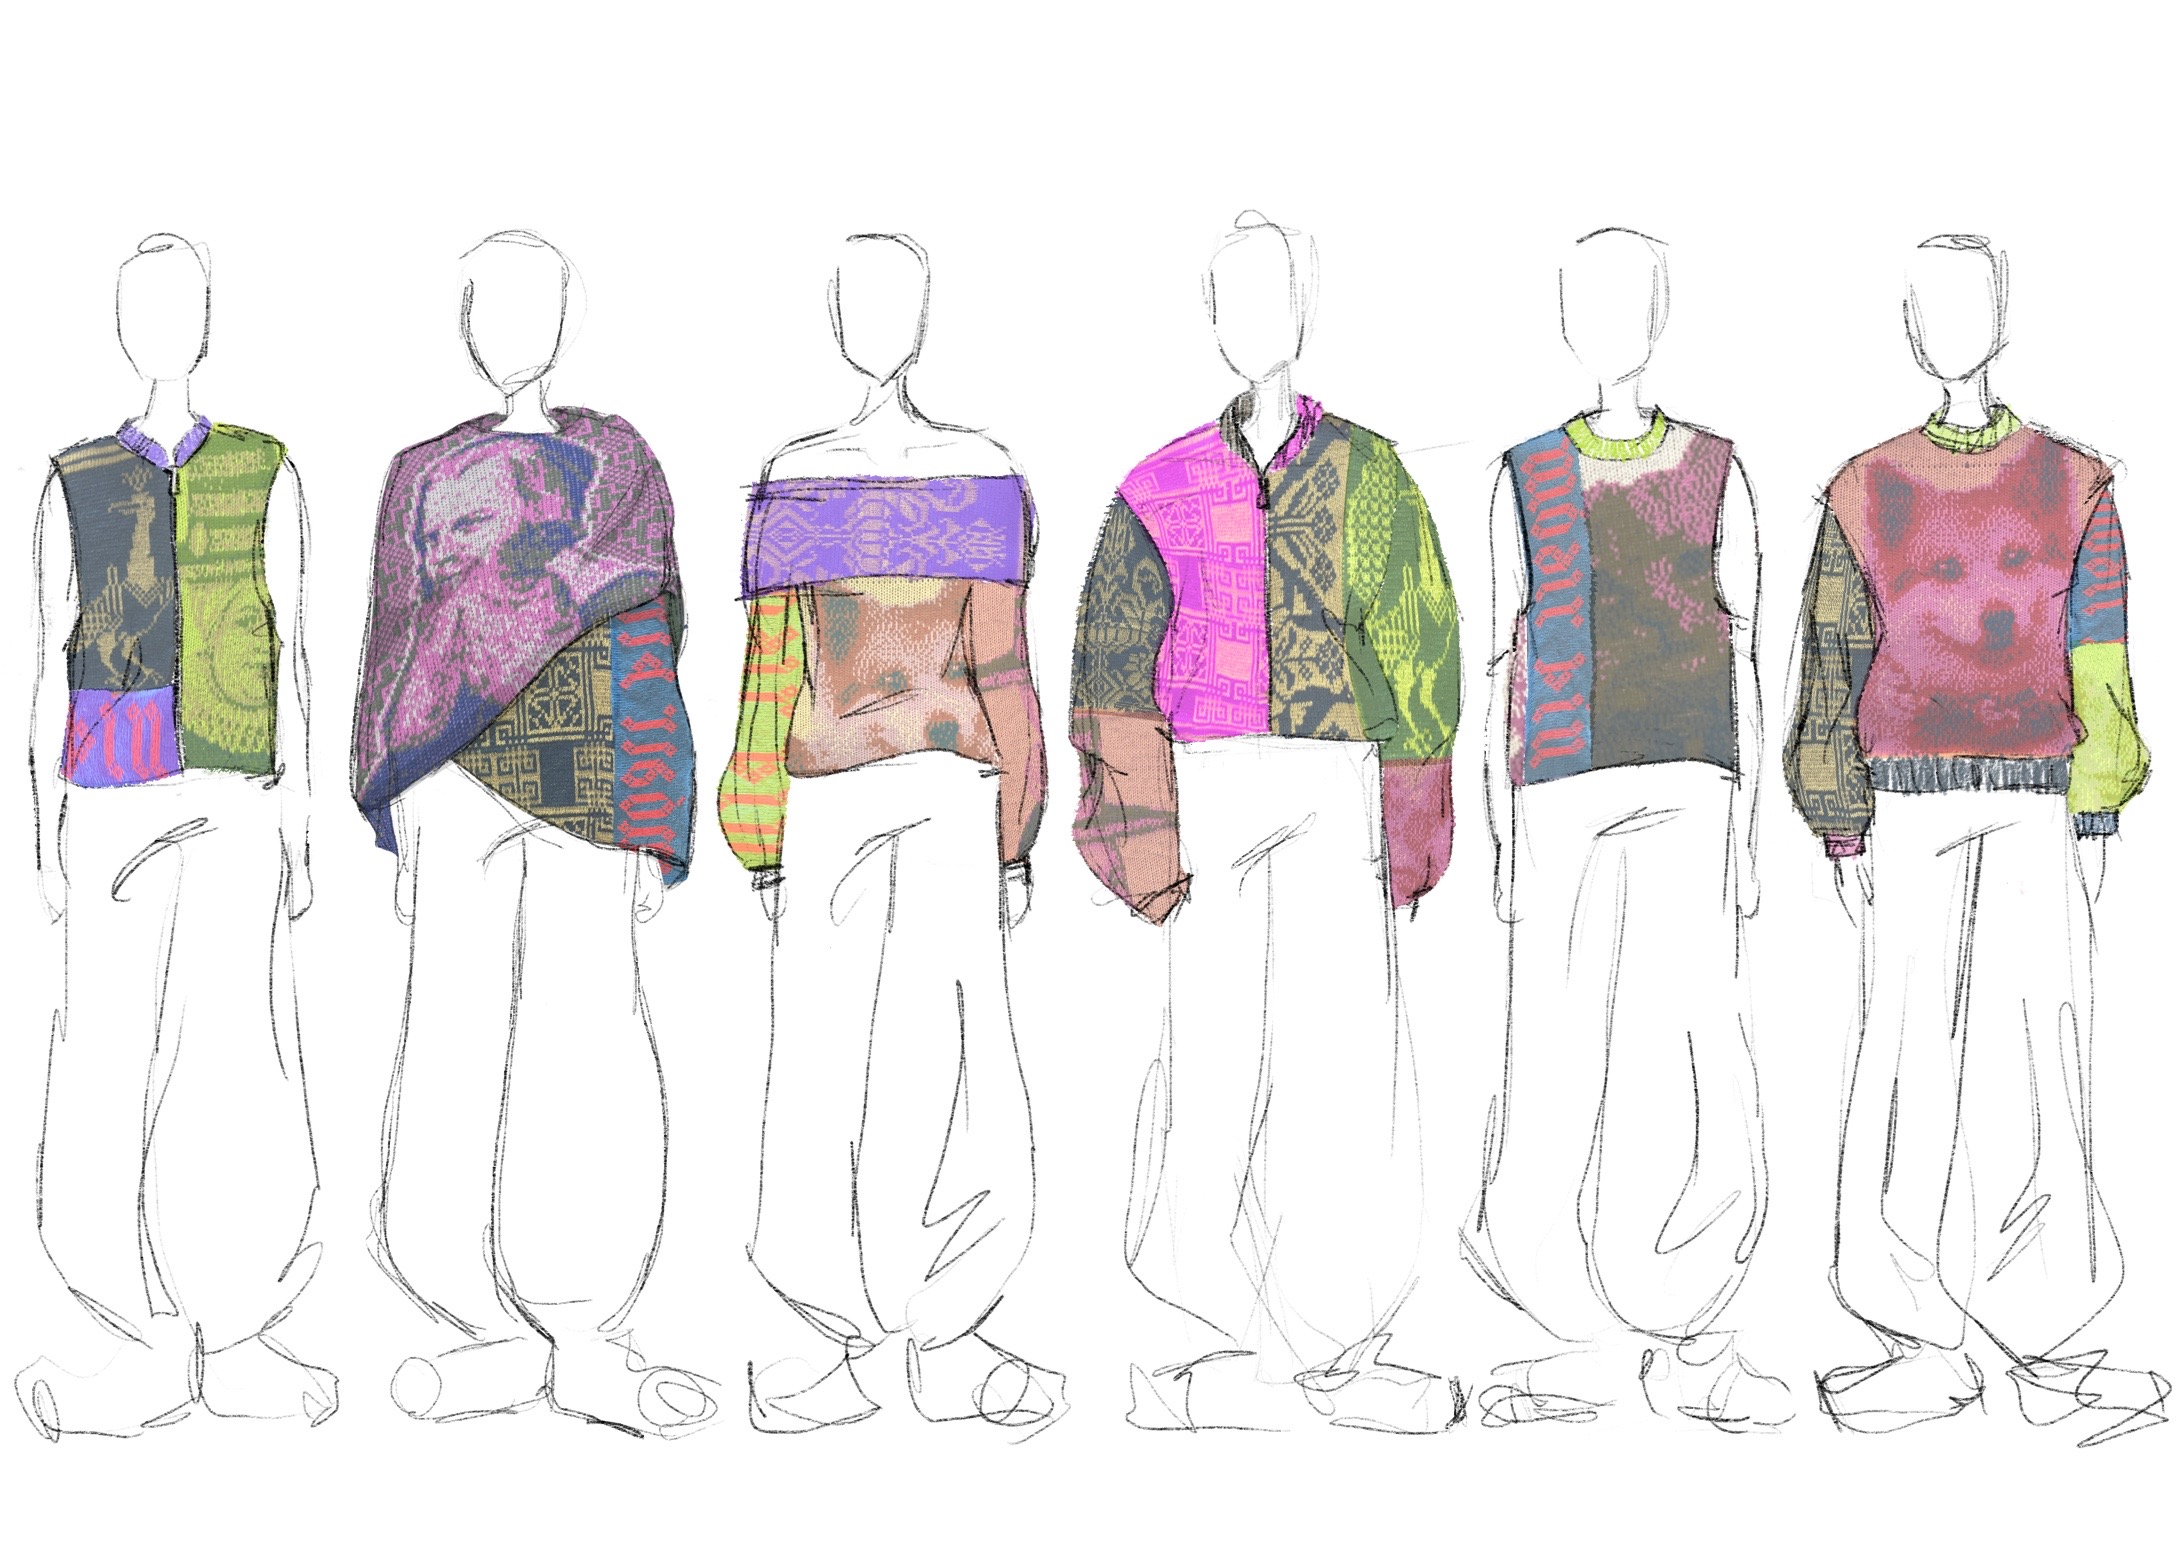
\includegraphics[width=\linewidth]{myndir/gisa/collection.JPG}
    \caption{Nokkrar útfærslur á fatnaði út frá prjónaprufum sumarsins.}
    \label{fig:designproposal}
\end{figure}

\subsubsection{Menningararfur og tenging við fortíðina}
Ragnheiður ,,yngri'' Jónsdóttir sem margir kannast eflaust við af 5.000kr seðlinum var mikil handverkskona og safnaði í sjónabók sem notuð var í mynstur í fyrsta kafla \textit{Sjónabókar} og er hún því áhrifamikil í menningararfi okkar Íslendinga. Á Þjóðminjasafni Íslands heillaðist hönnuður af henni og hennar mynstrum og ákváðum við því að heiðra framlag hennar með því að prjóna mynd af henni. Þessi prufa var byltingarkennd í ferlinu og má sjá mynd af henni, 50 lykkjur á breidd og aðra, 120 lykkjur á breidd á mynd \ref{fig:ragga:knit}. Í framhaldinu fórum við að blanda saman myndum og mynstrum og þannig tengja menningararf okkar inn í nútíma hönnun með því að blanda nútíð og fortíð saman. Hallgrímskirkja var ein þeirra eins og má sjá á mynd \ref{fig:hallgrimskirkja}. Náin samvinna tölvunarfræðinema og hönnuðar var lykilatriði í framvindu verkefnisins og býður upp á marga ókannaða möguleika. 

\begin{figure}[p]
    \centering
    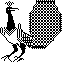
\includegraphics[height=.20\textheight]{myndir/thjms5898_246_0.png}
    \hspace{24pt}
    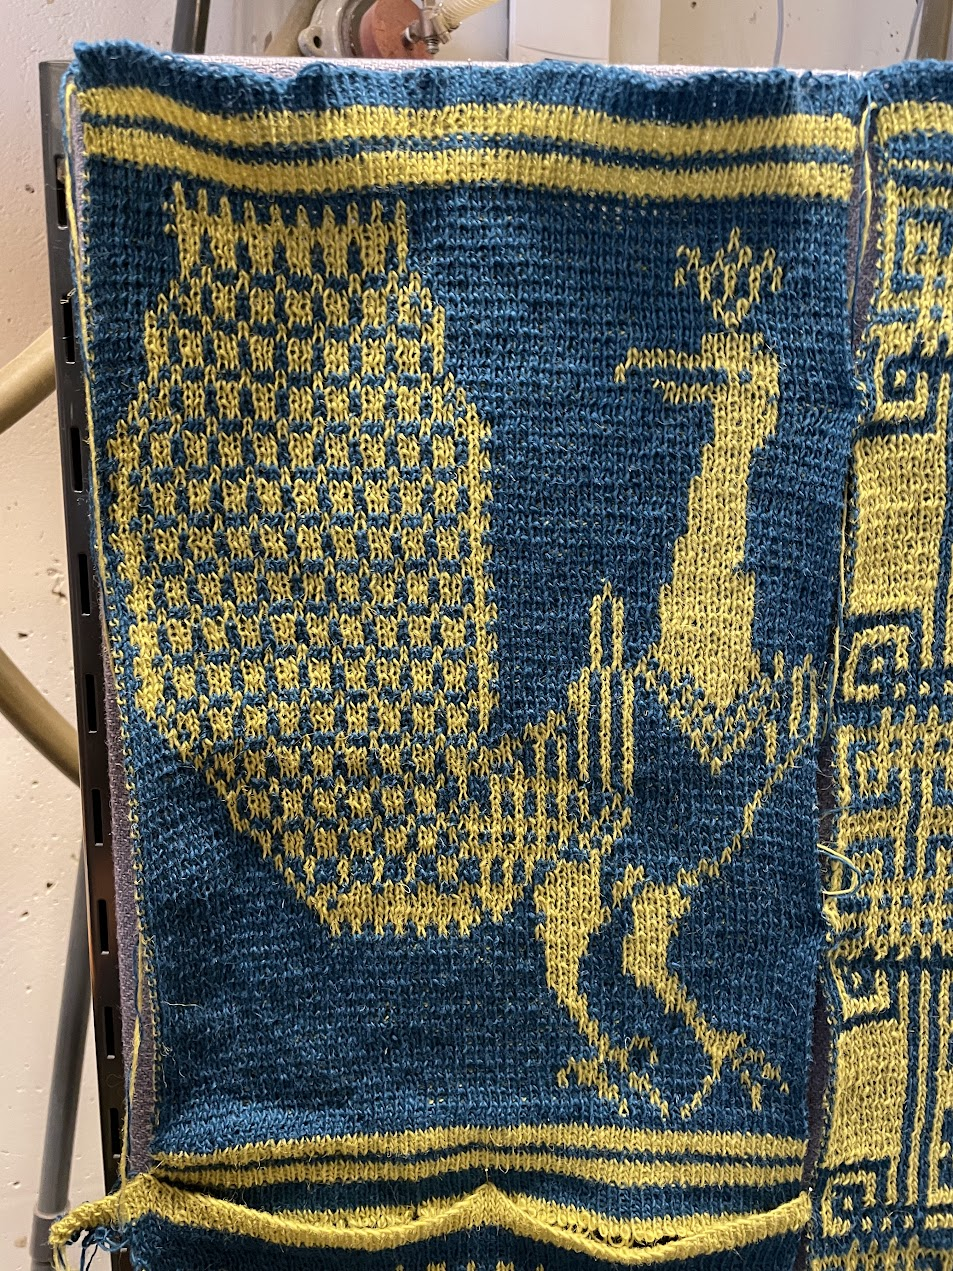
\includegraphics[height=.20\textheight]{myndir/peacock.jpg}
    \caption{Páfugl, bls. 246 í Sjónabók (Þjms. 5898)}
    \label{fig:peacock}
\end{figure}

\begin{figure}[p]
    \centering
    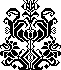
\includegraphics[height=.20\textheight]{myndir/thjms5898_210.png}
    \hspace{24pt}
    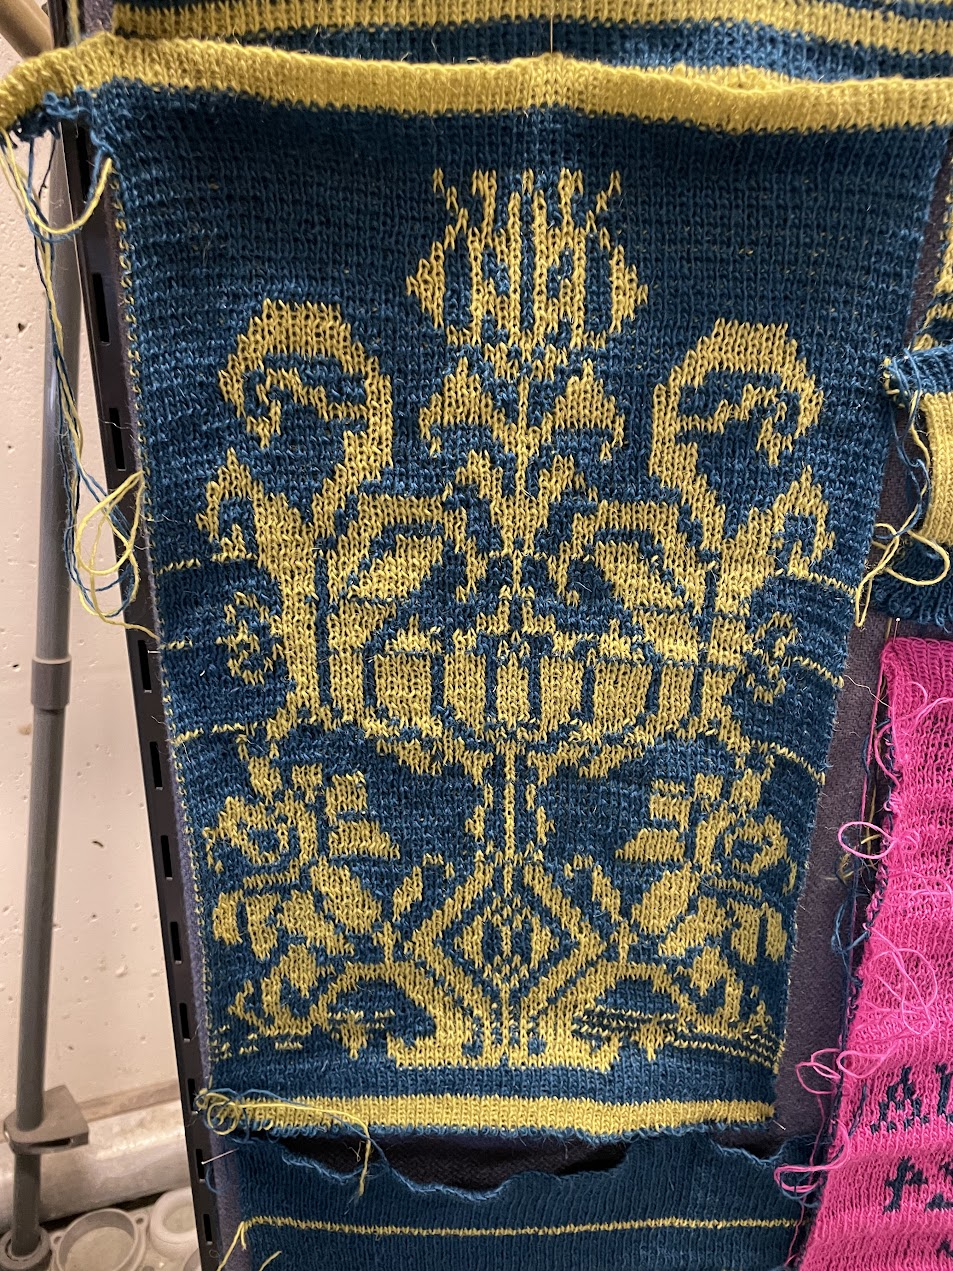
\includegraphics[height=.25\textheight]{myndir/flower.jpg}
    \caption{Blóm, bls. 210 í Sjónabók (Þjms. 5898)}
    \label{fig:flower}
\end{figure}

\begin{figure}[p]
    \centering
    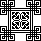
\includegraphics[height=.20\textheight]{myndir/thjms5898_268.png}
    \hspace{24pt}
    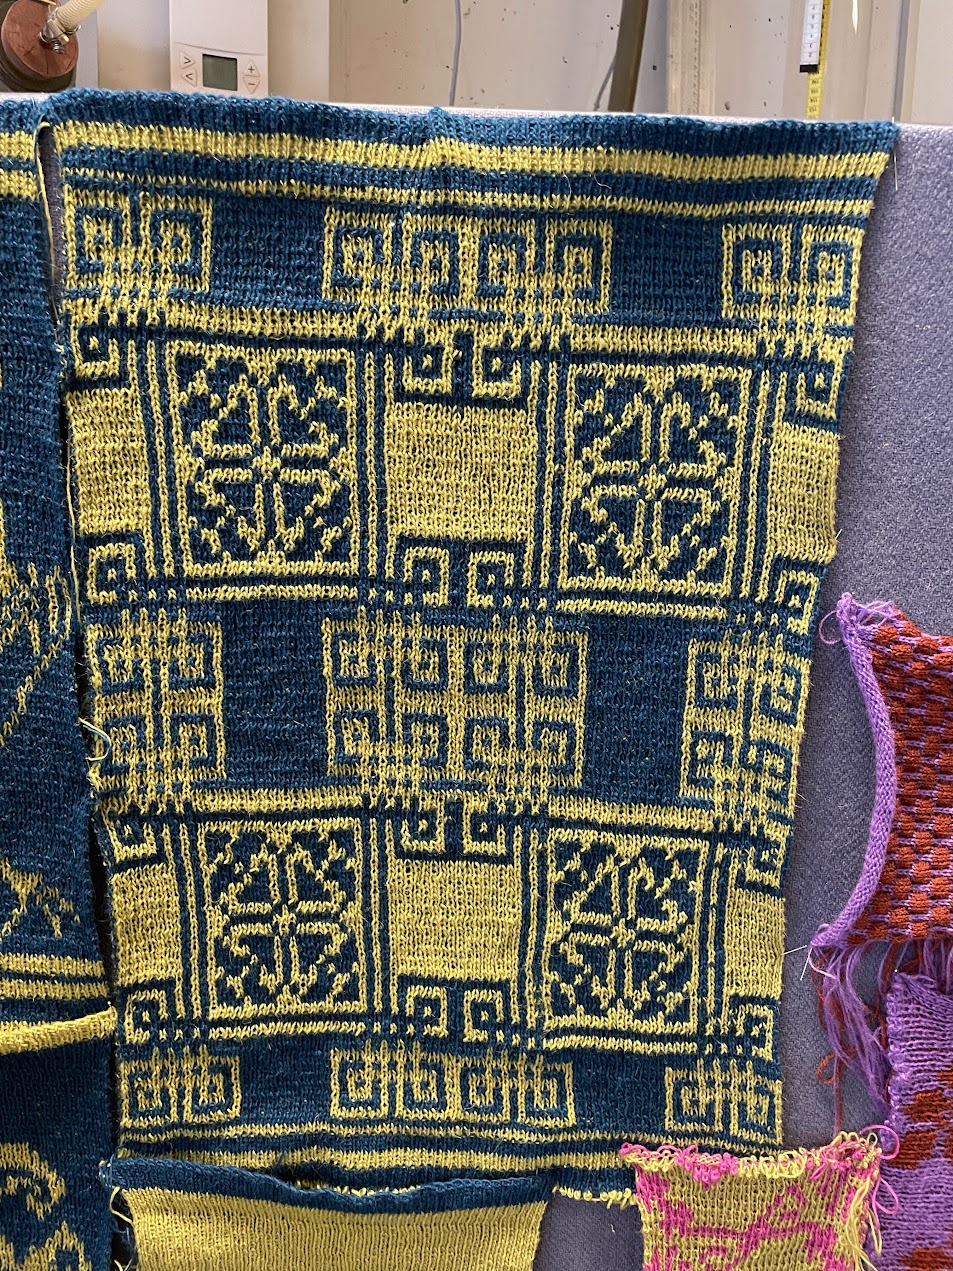
\includegraphics[height=.25\textheight]{myndir/repeat.jpg}
    \caption{Endurtekið mótif, bls. 268 í Sjónabók (Þjms. 5898)}
    \label{fig:repeat}
\end{figure}

\begin{figure}[p]
    \centering
    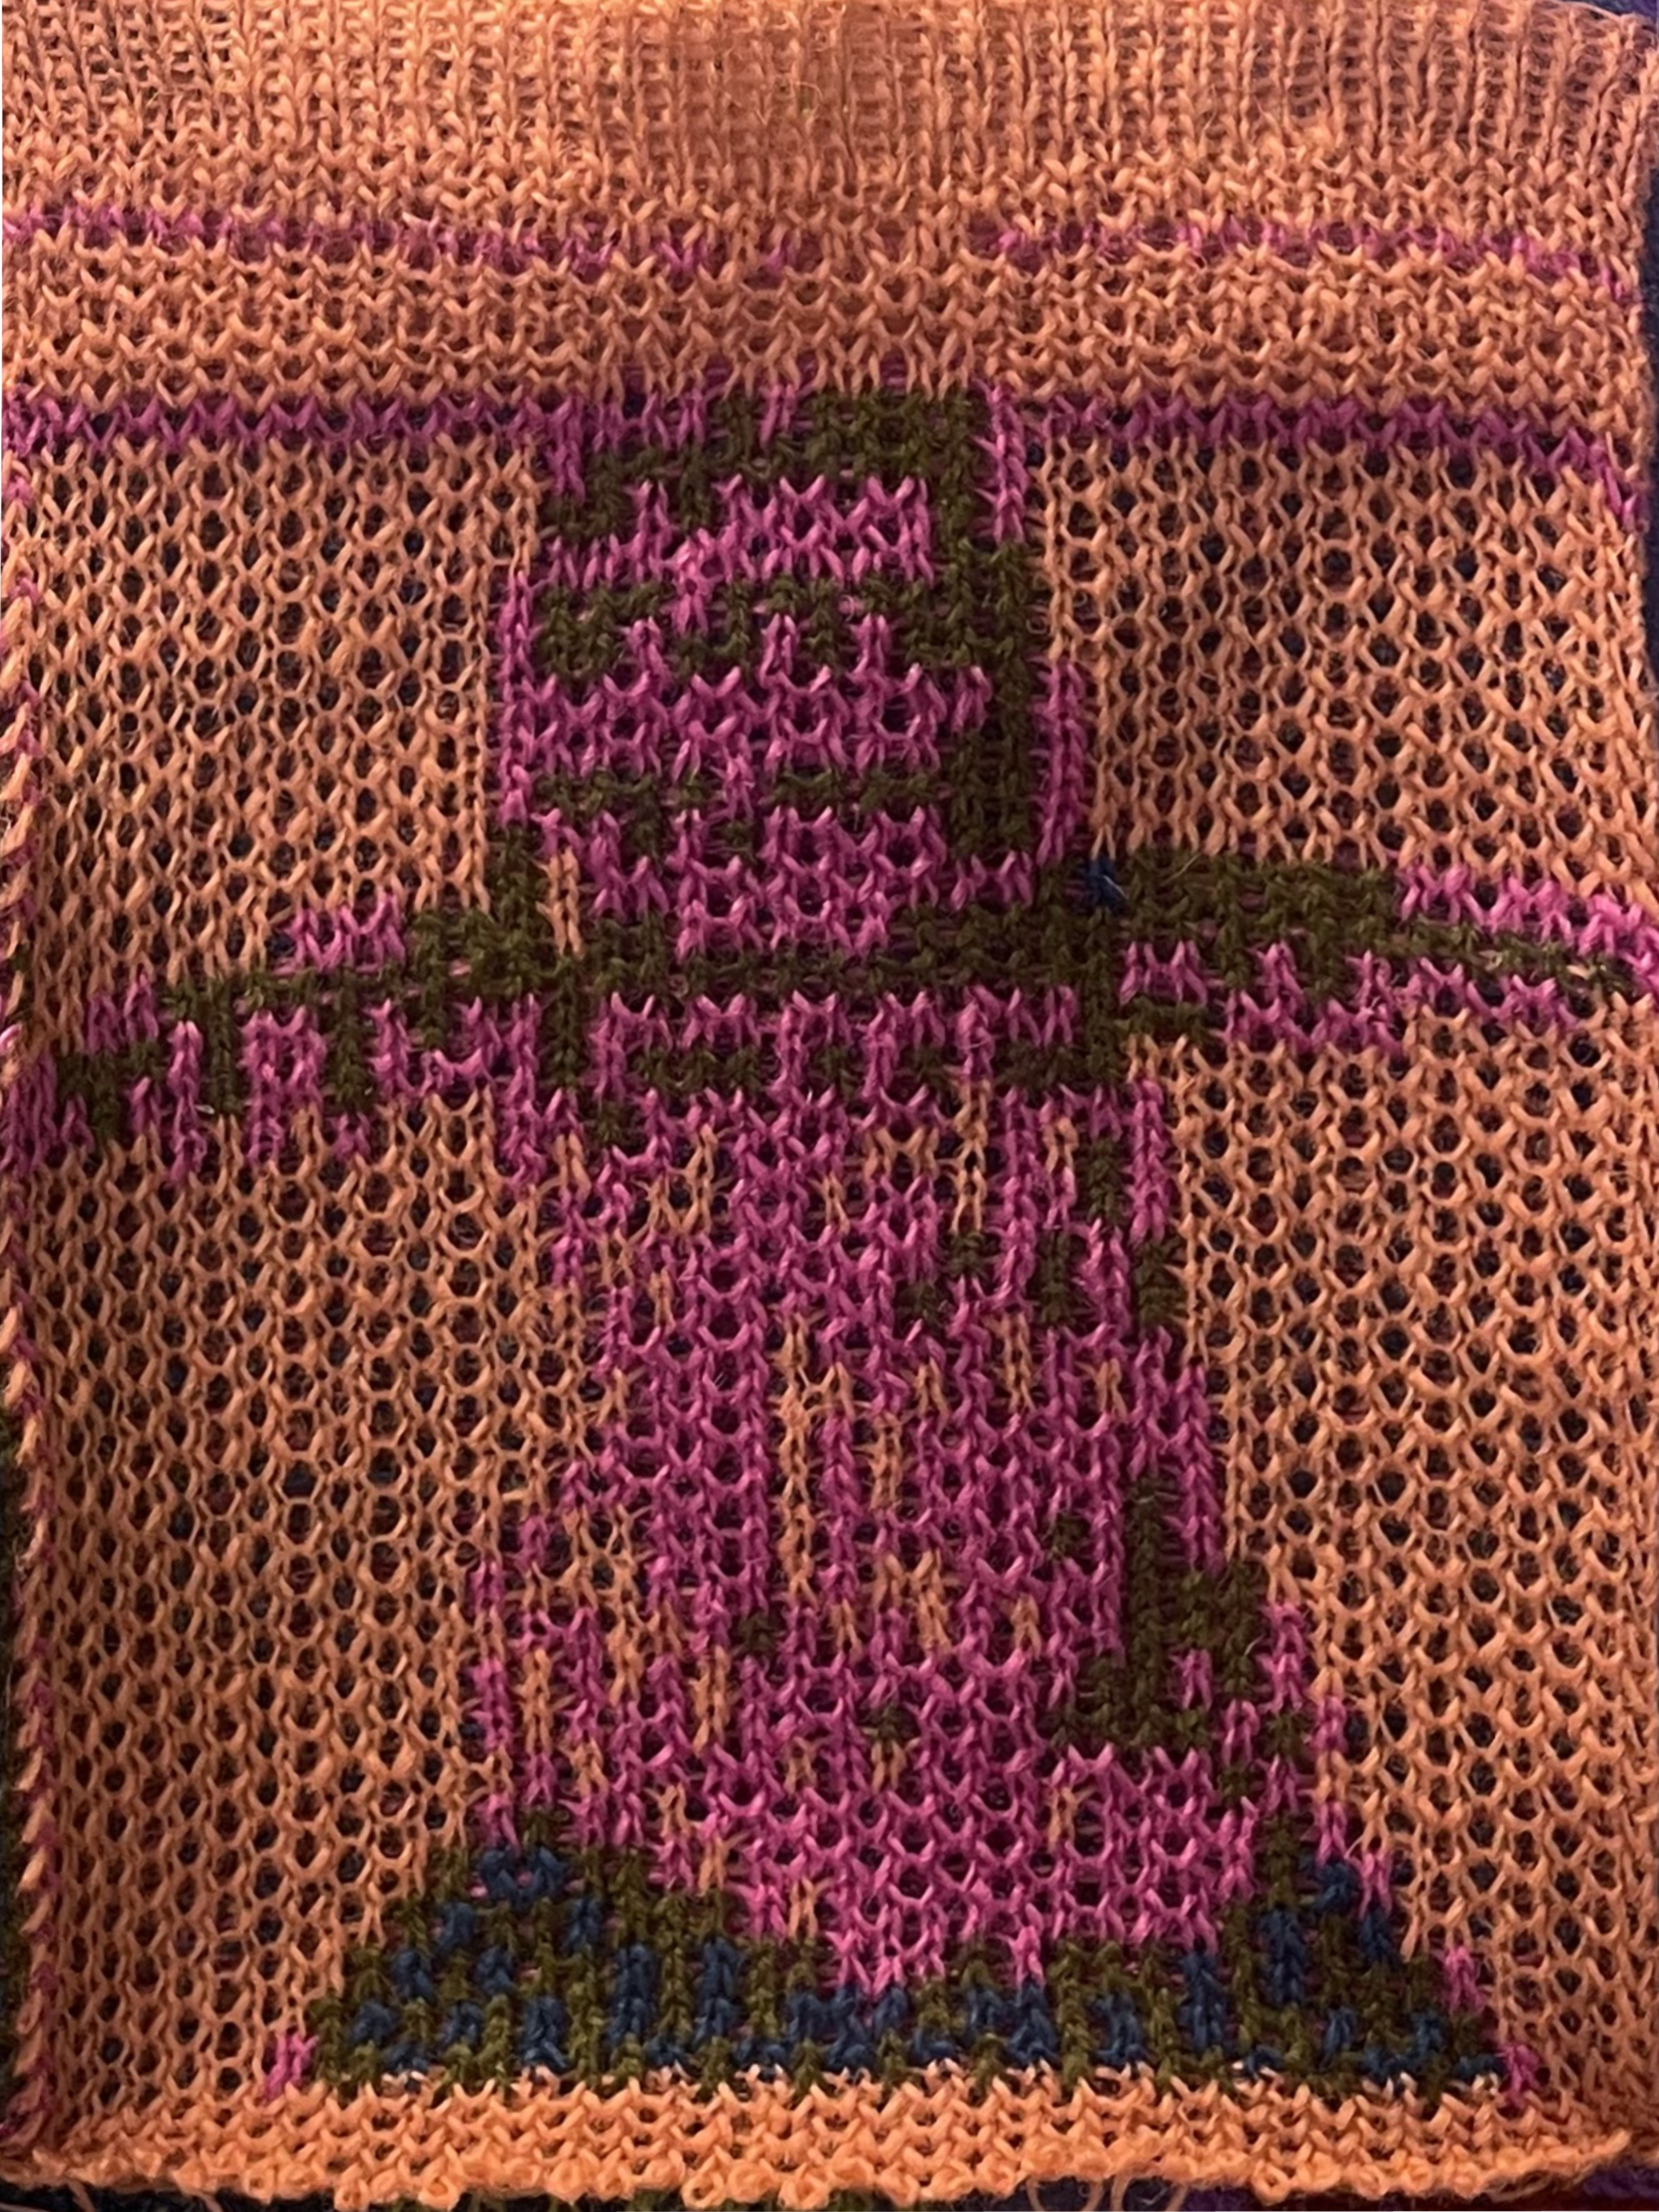
\includegraphics[height=.30\textheight]{myndir/gisa/ragga-lowres.JPG}
    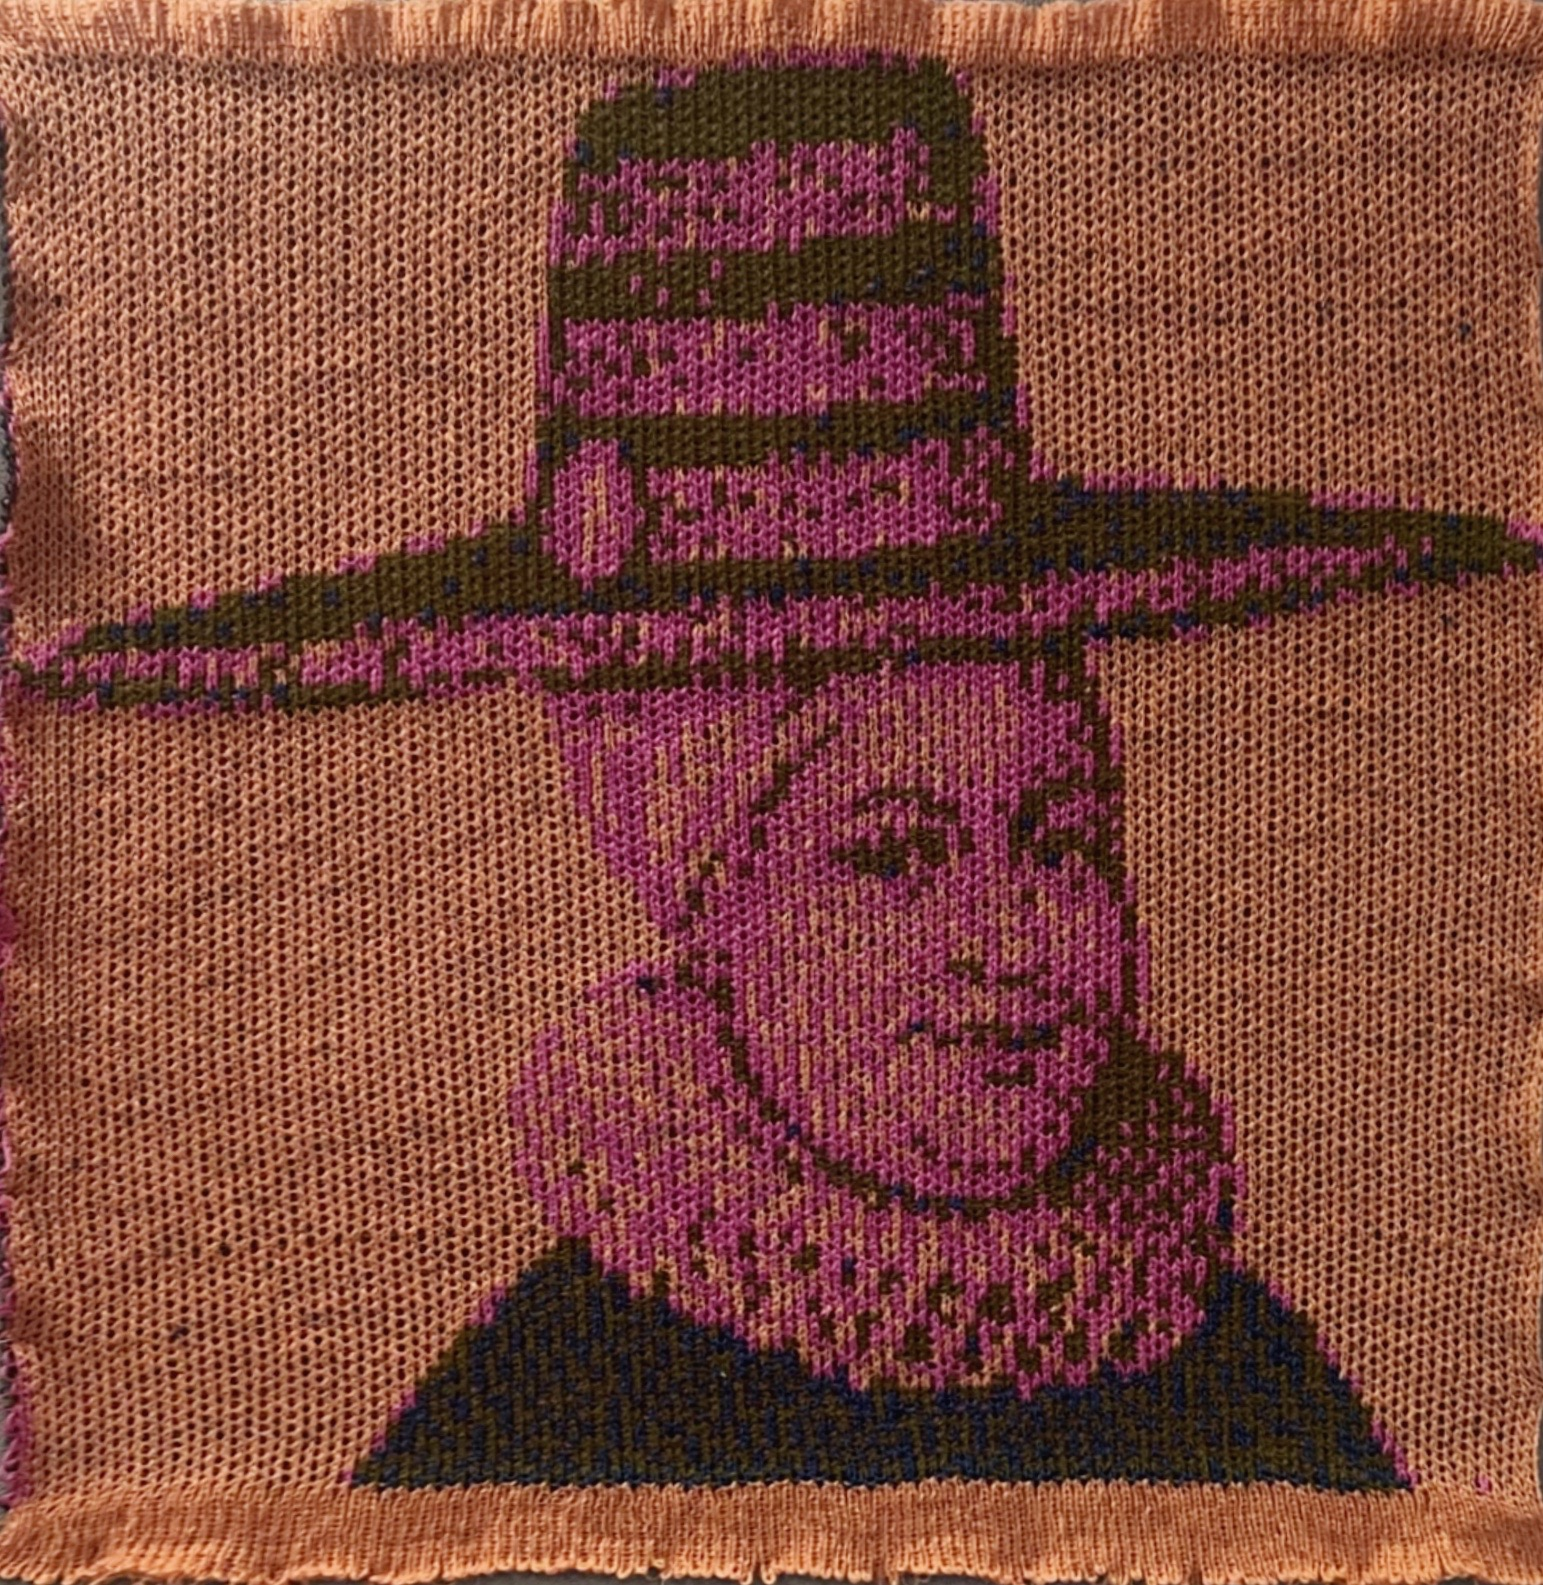
\includegraphics[height=.30\textheight]{myndir/gisa/ragga-hires.JPG}
    \caption{Ragnheiður ,,yngri'' Jónsdóttir: 50 lykkjur á breidd (til vinstri) og 120 lykkjur á breidd (til hægri).}
    \label{fig:ragga:knit}
\end{figure}

\begin{figure}[p]
    \centering
    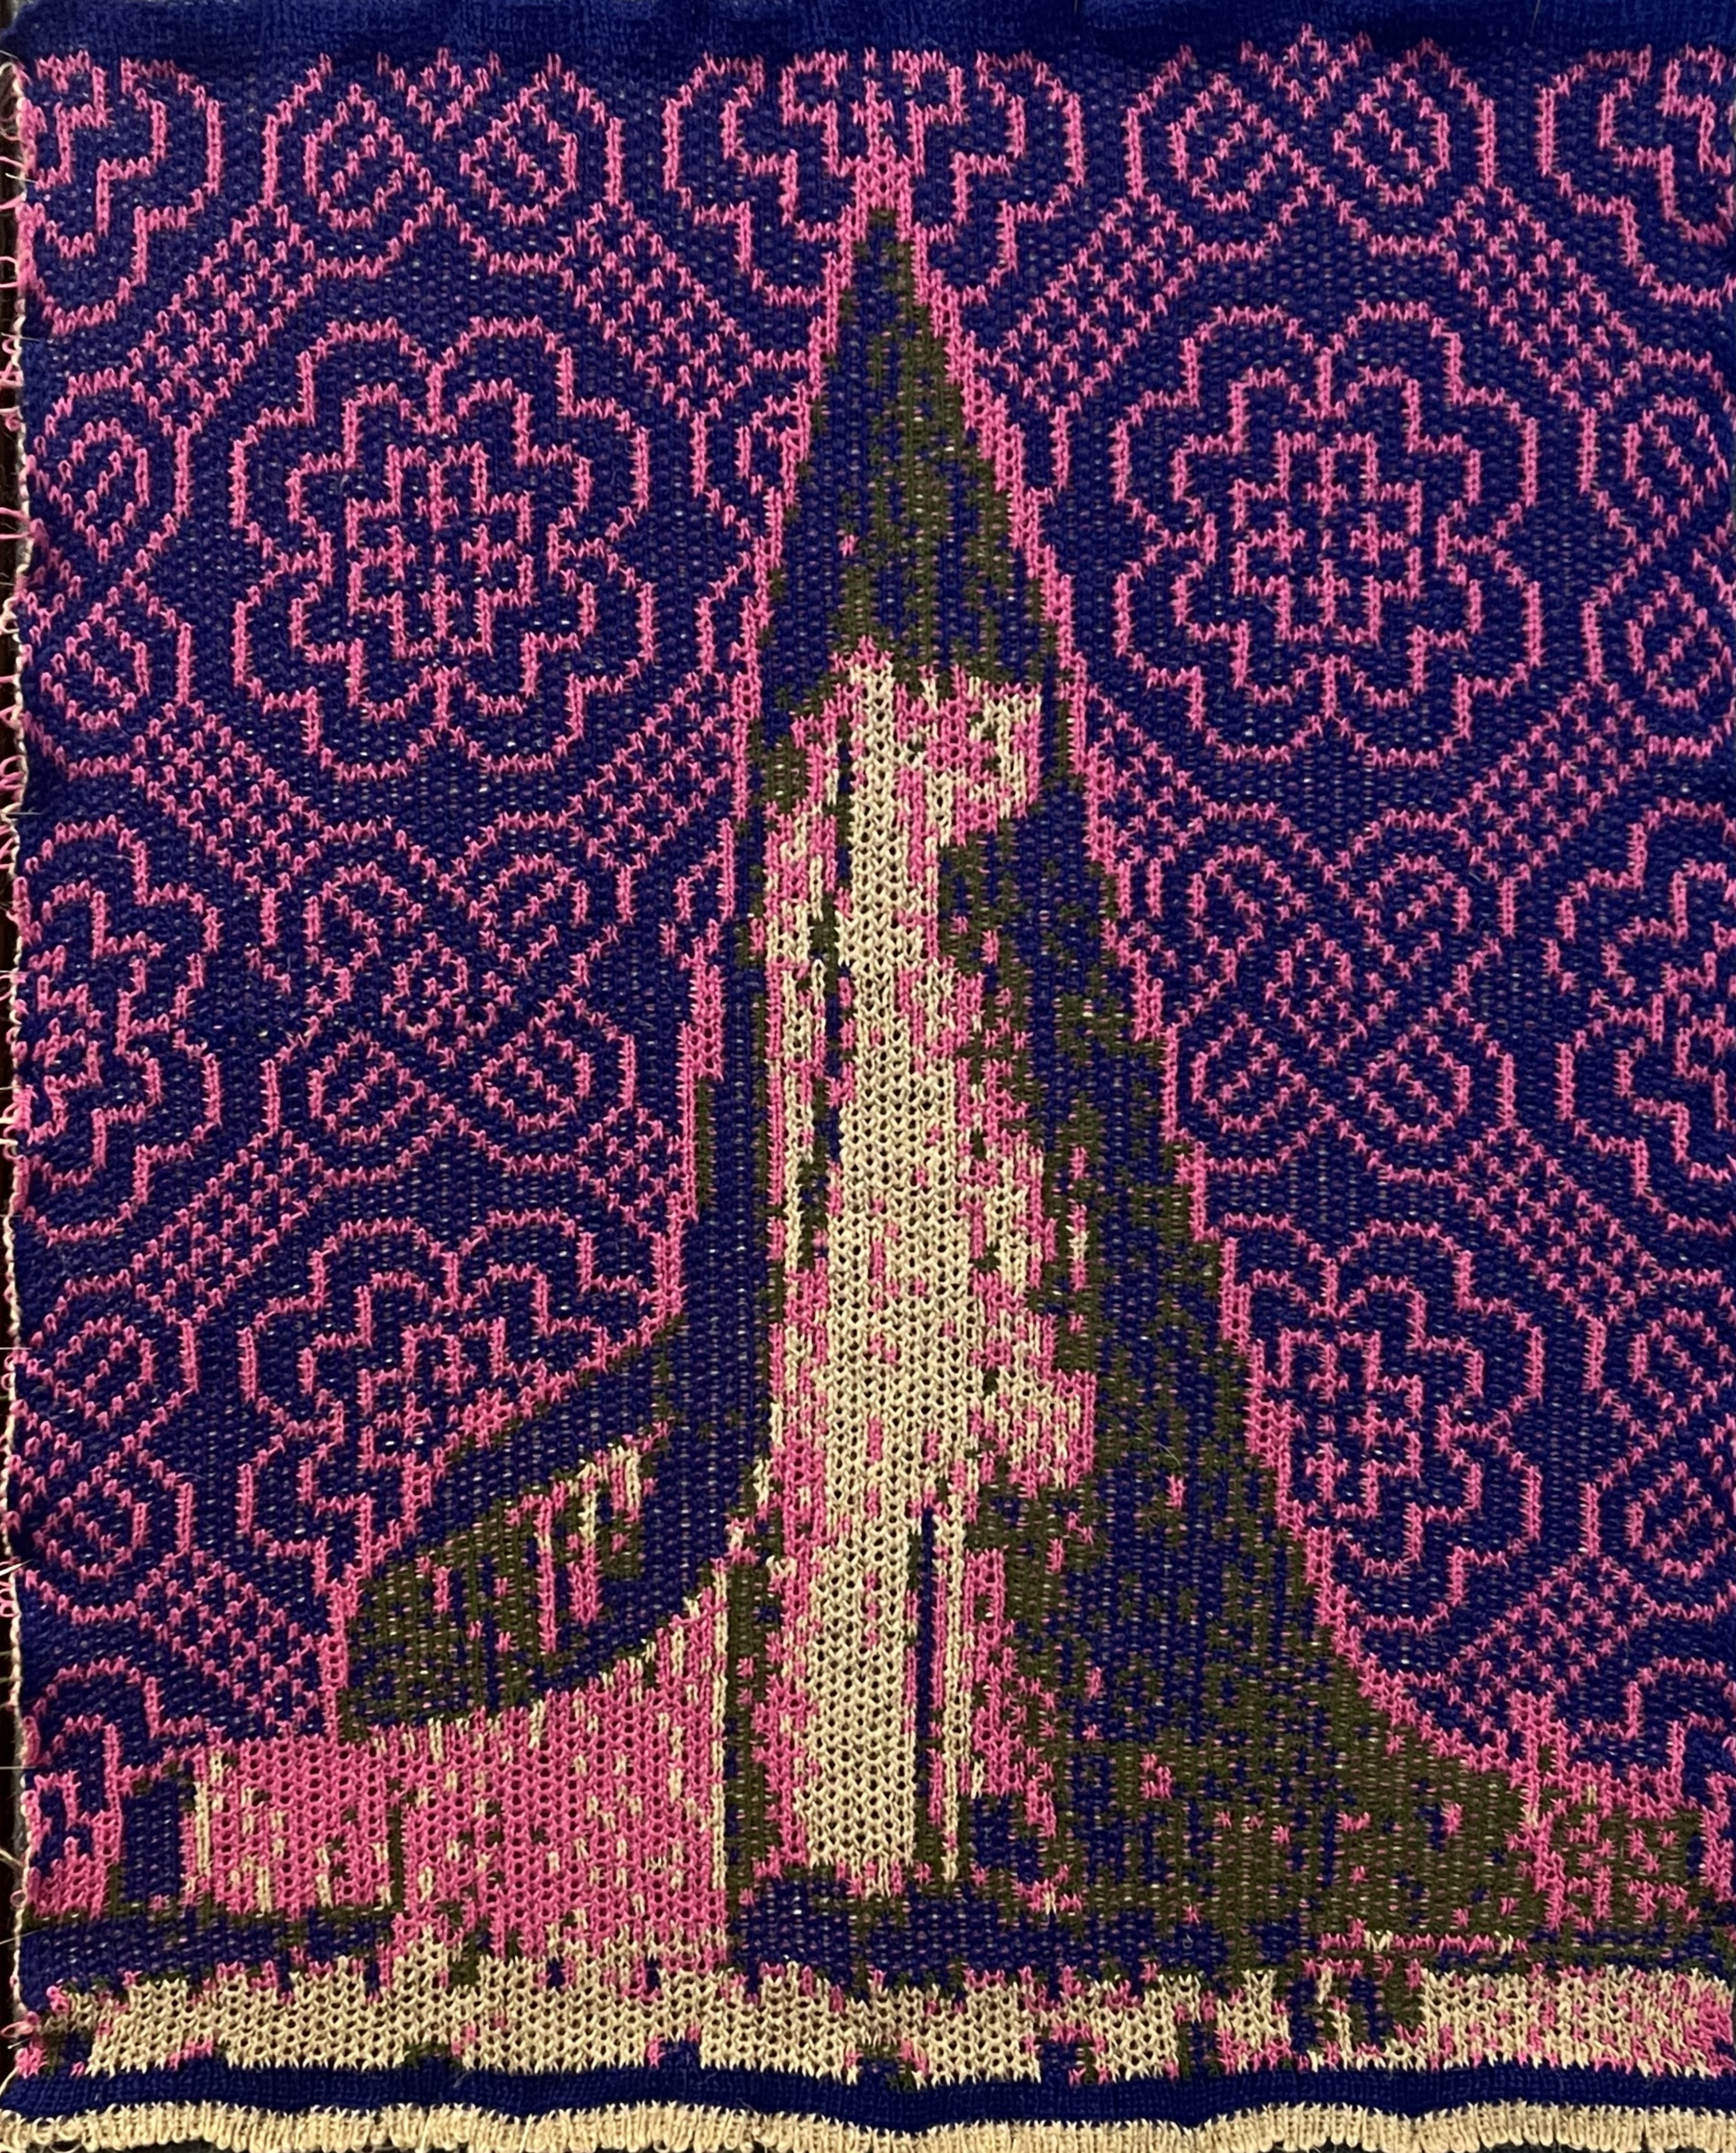
\includegraphics[height=.5\textheight]{myndir/gisa/hallgrimskirkja.JPG}
    \caption{Hallgrímskirkja}
    \label{fig:hallgrimskirkja}
\end{figure}